%\vspace{-10pt}
%
%In this section we evaluate performance of Algorithms \ref{alg:asym} and \ref{alg:UCB} on synthetic and real datasets. For synthetic example, we consider data transmission over a binary symmetric channel, and for real world examples, we use diabetes (PIMA indiana) and heart disease (Clevland) from UCI dataset. In both datasets attributes/features are associated with costs, where features related to physical observations are cheap and that obtained from medical tests are costly. The experiments are setup as follows:
%
%{\bf Synthetic:} we consider data transmission over three binary symmetric channels (BSCs). Channel $i=1,2,3$ flips input bit with probability $p_i$ where $p_1\geq p_2\geq p_3$. Transmission over channel $1$ is free and that over channel $2$ and $3$ costs price of $ c_2$ and $c_3\in (0,1] $ units per bit, respectively. Input bits are generated with probability $0.7$ and we set $p_1=.4, p_2=.1$ and $p_3=.05$.
%
%{\bf Datatsets:} we obtain a sensor acquisition setup from the datasets as follows: Three svm classifiers (linear, $C=.01$) are trained for each dataset, first one using only cheap features, second one  using cheap features plus few additional features and the third one using all features. These classifiers form sensors of a three stage SAP where classifier trained with cheap features is the first stage and that trained with all the features forms the last stage. Cost of each stage is the sum of cost of features used to train that stage multiplied by a scaling factor $\lambda$ (trade-off parameter between prediction accuracy and costs). Specific details for each dataset is given below.  
%
%{\bf PIMA indians diabetes} dataset consists of $768$ instances and has $8$ attributes. The labels identify if the instances are diabetic or not. First sensor of SAP is trained with $4$ cheap attributes and costs \$$4$ (times-pregency, pedigree, diastolic-pb, triceps ). Second sensor is trained from $7$ attributes that includes age, mass-index and insulin in addition to the attributed used for the first sensor and cost total of \$$29$, and the last sesnor is trained with all $8$ attributes that cost \$$46$. We set $C_1= 4\lambda, C_2= 29\lambda$ and $C_3= 46\lambda$.
%% $6$ of the attributes obtained from physical observations are cheap, and $2$ attributes (glucose and insulin) require expensive tests. 
%
%{\bf Heart disease} dataset consists of $297$ instance (without missing values) and has $13$ attributes. $5$ class labels $(0,1,2,3,4)$ are mapped to binary values by taking value $0$ as `absence' of disease and values $(1,2,3,4)$ as `presence' of disease. First senor of SAP is trained with first $7$ attributes which cost  \$$32$ in total, second sensor is trained with first $11$ attributes that cost \$$1$ each and the third sensor is trained with all the attributes  cost total of \$$568$. We set $C_1= 32\lambda, C_2= 397\lambda$ and $C_3= 601\lambda$.
%=======
%\begin{figure*}[!bt]
%	\begin{minipage}{4cm}
%		\centering
%		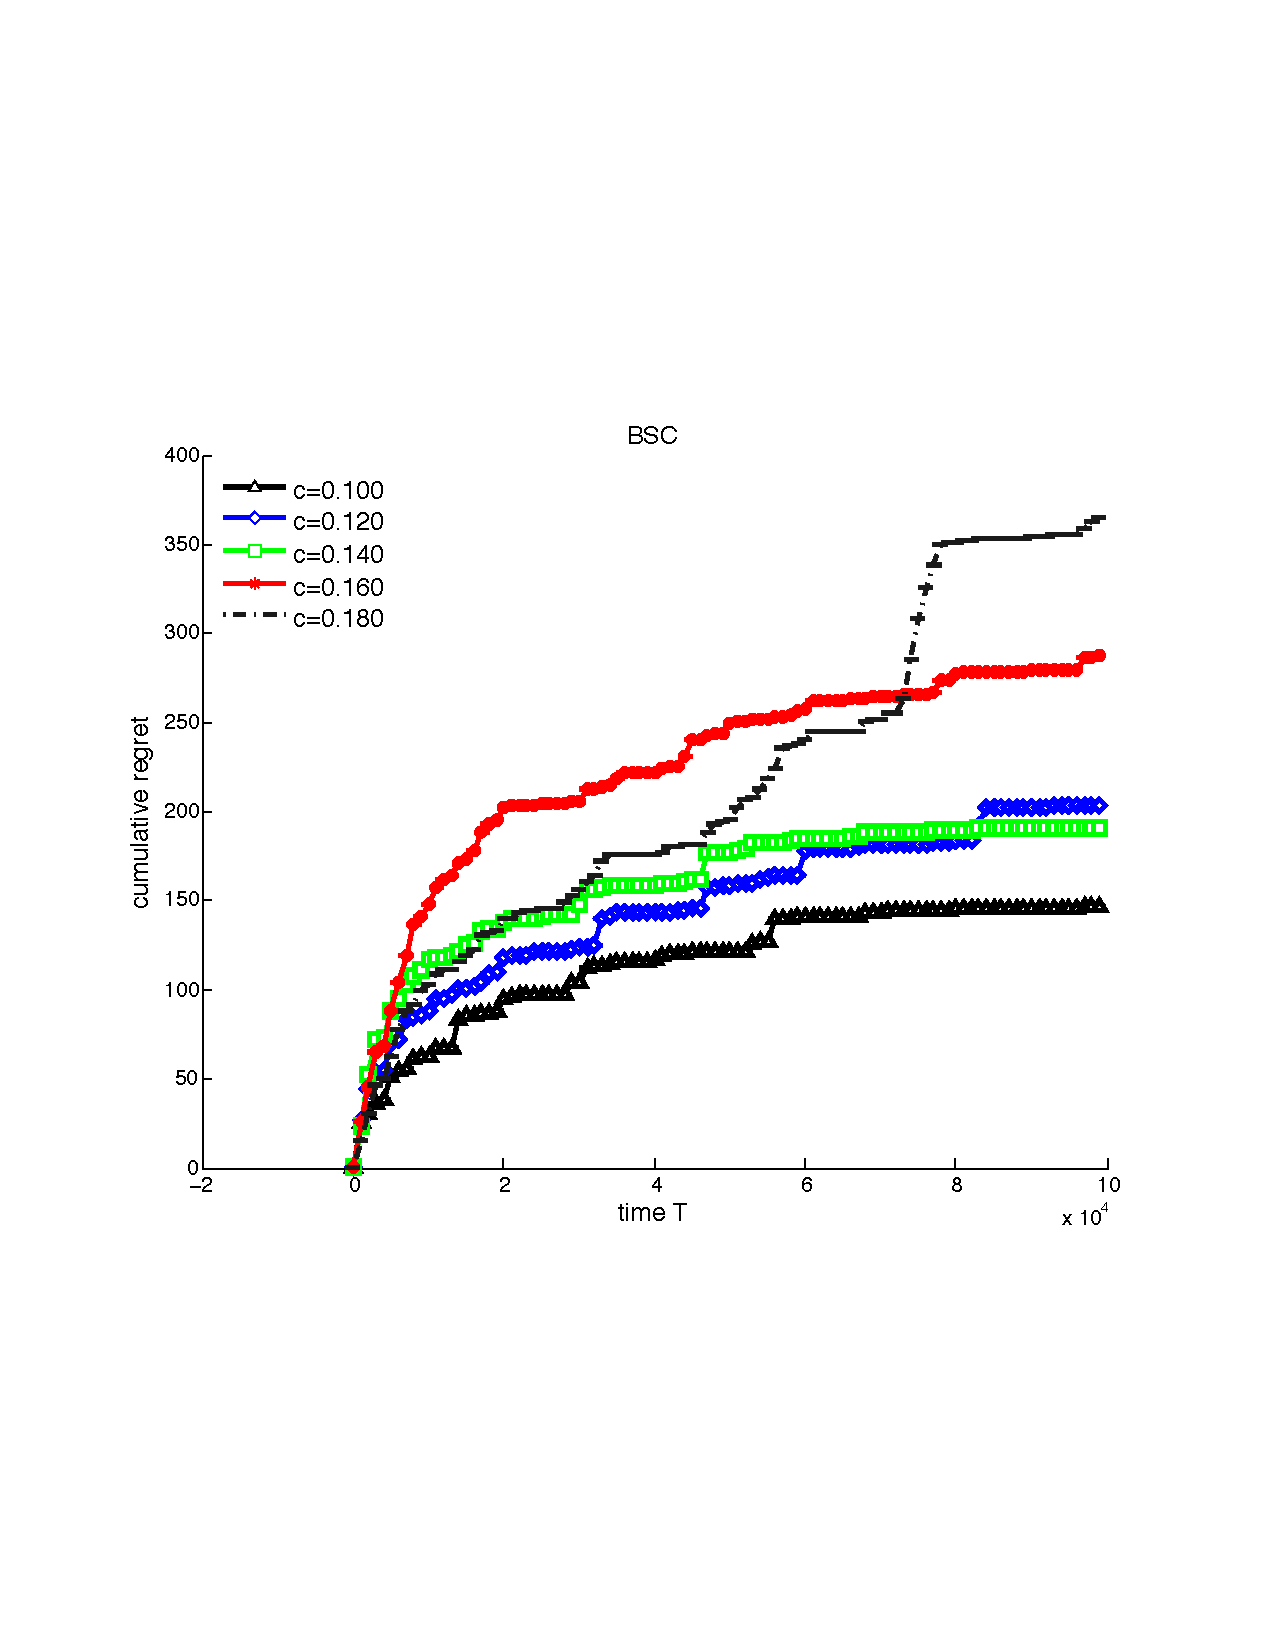
\includegraphics[scale=0.2]{../Simulations/Figures/BSC_SD}
%		\label{fig:BSC1}
%		\caption{BSC wtih SD}
%	\end{minipage}
%	\begin{minipage}{4cm}
%		\centering
%		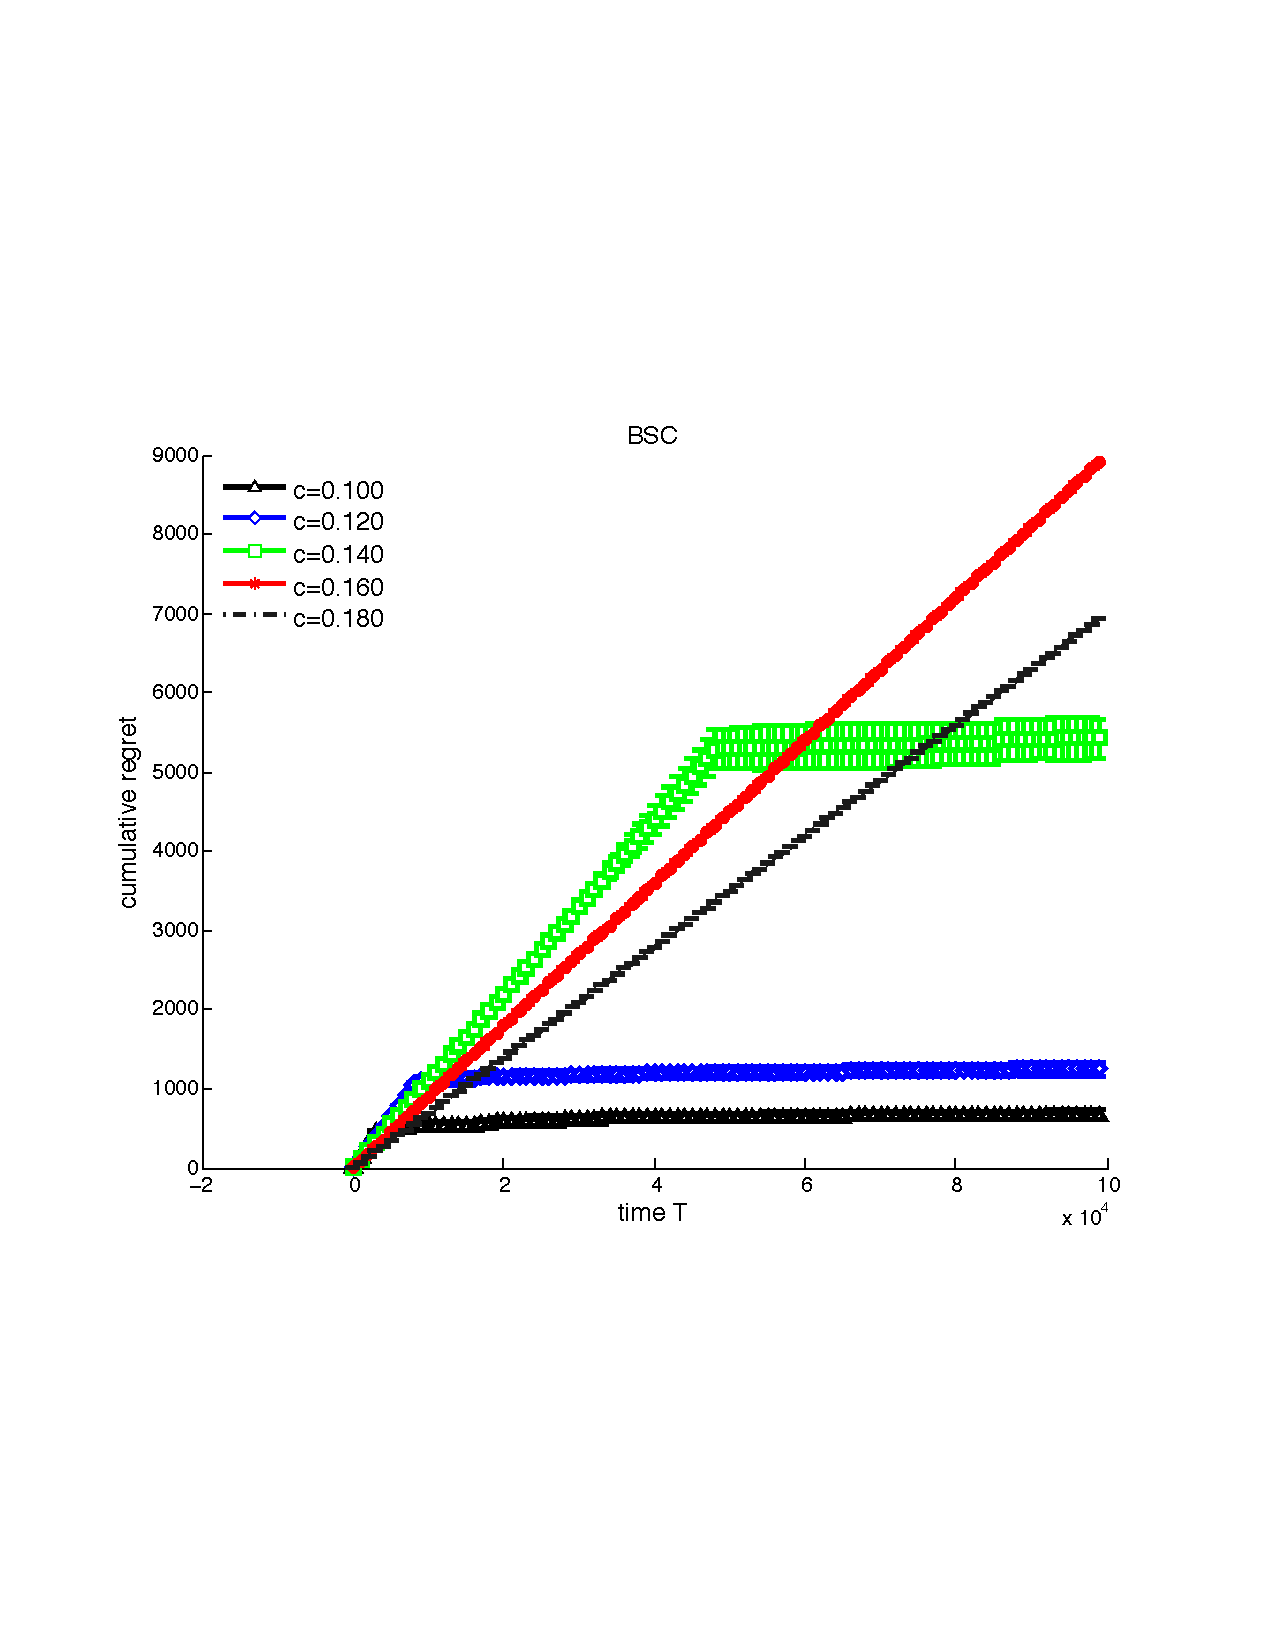
\includegraphics[scale=0.2]{../Simulations/Figures/BSC_WD}
%		\label{fig:BSC2}
%		\caption{BSC dataset}
%	\end{minipage}
%	\begin{minipage}{4cm}
%		\centering
%		\includegraphics[scale=0.2]{../Simulations/Figures/Heart}
%		\label{fig:Heart}
%		\caption{BSC dataset}
%	\end{minipage}
%	\begin{minipage}{4cm}
%		\centering
%		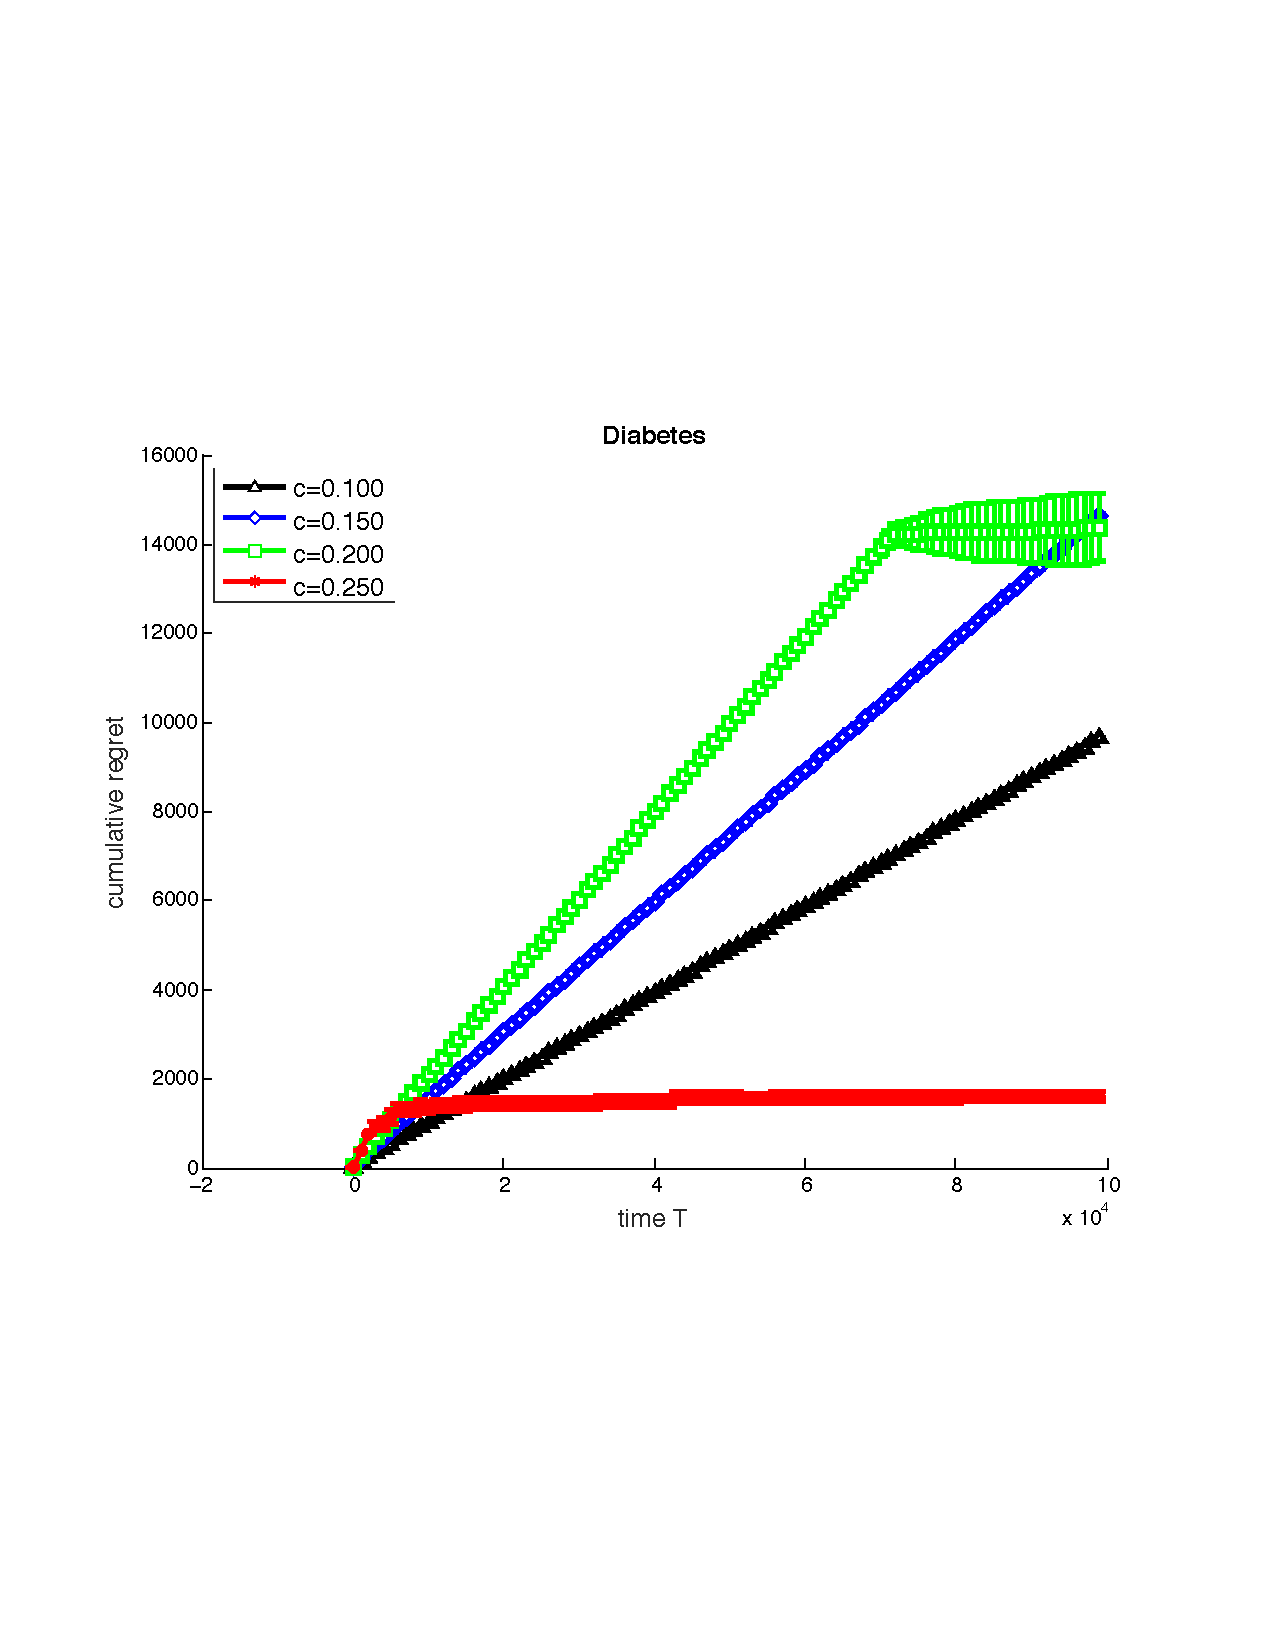
\includegraphics[scale=0.2]{../Simulations/Figures/Diabetes_WD}
%		\label{fig:Heart}
%		\caption{Heart dataset}
%	\end{minipage}
%	\vspace{.2cm}

%\noindent
%In Fig. \ref{fig:BSC1}, BSC data is generated that satisfies SD property and Algorithm \ref{alg:asym} is applied. In  Fig. \ref{fig:BSC2}, Algorithm \ref{alg:UCB} is applied on BSC data. In Fig. \ref{fig:BSC3}, true labels are used and standard UCB algorithm is applied on BSC dataset. In Fig. \ref{fig:Heart}, we applied Algorithm \ref{algo:UCB} on the heart dataset. 
%\end{figure*}
%
In this section we evaluate performance of Algorithms \ref{alg:asym} and \ref{alg:UCB} on synthetic and real datasets (PIMA-Diabetes) and Heart Disease (Cleveland). Both of these datasets have accompanying costs for individual features.%. For synthetic example, we consider a binary symmetric channel, and for real world examples, we use diabetes (PIMA indiana) and heart disease (Clevland) from UCI dataset. In both datasets attributes/features are associated with costs, where features related to physical observations are cheap and that obtained from medical tests are costly. The experiments are setup as follows:

{\bf Synthetic:} We generate data as follows. The input, $Y_t$, is generated IID Ber($0.7$). Outputs for channels 1, 2, 3 have an overall error statistic, $\gamma_1 = 0.4,\,\gamma_2=0.1,\,\gamma_3=0.05$ respectively. To ensure SD we enforce Defn.~\ref{eqn:DominanceCondition} during the generation process. To relax SD requirement we introduce errors upto 10\% during data generation for sensor outputs 2 and 3 when sensor 1 predicts correctly.% (while still maintaint the overall error).  

%Channel $i=1,2,3$ flips input bit with probability $p_i$ where $p_1\geq p_2\geq p_3$. Transmission over channel $1$ is free and that over channel $2$ and $3$ costs price of $ c_2$ and $c_3\in (0,1] $ units per bit, respectively. Input bits are generated with probability $0.7$ and we set $p_1=.3, p_2=.1$ and $p_3=.05$.

{\bf Real Datasets:} %we obtain a sensor acquisition setup from the datasets as follows: 
We split the features into three ``sensors'' based on their costs. For PIMA-Diabetes dataset (size=$768$) the first sensor is associated with patient history/profile with cost (\$6), the 2nd sensor in addition utilizes  insulin test (cost \$ 22) and the 3rd sensor uses all attributes (cost \$46). For the Heart dataset (size=$297$) we use the first $7$ attributes that includes cholestrol readings, blood-sugar, and rest-ECG (Cost \$27), the 2nd sensor utilizes in addition thalach, exang, oldpeak attributes that cost $\$300$  and the 3rd sensor utilizes more extensive tests at a total cost of \$601. 


We train three linear SVM classifiers with 5-fold cross-validation and have verified that our results match known state-of-art. Note that Table~\ref{tab:ErrorTable1} shows that the resulting classifiers/tests on these datasets approximately satisfies SD condition and thus our setup should apply to these datasets. 
%
%
%The (linear, $C=.01$) are trained for each dataset, first one using only cheap features, second one  using cheap features plus few additional features and the third one using all features. These classifiers form sensors of a three stage SAP where classifier trained with cheap features is the first stage and that trained with all features forms the last stage. Cost of each stage is the sum of cost of features used to train that stage multiplied by a scaling factor $\lambda$ (trade-off parameter for accuracy and costs). Specific details for each dataset is given below.  
%
%{\bf PIMA indians diabetes} dataset consists of $768$ instances and has $8$ attributes. The labels identify if the instances are diabetic or not. $6$ of the attributes (age, sex, triceps, etc.) obtained from physical observations are cheap, and $2$ attributes (glucose and insulin) require expensive tests. First sensor of SAP is trained with $4$ cheap attributes and costs \$$4$. Second sensor is trained from $6$ attributes that cost \$$6$, and the last sesnor is trained with all $8$ attributes that cost \$$6$. We set $C_1= 4\lambda, C_2= 6\lambda$ and $C_3= 30\lambda$.
%
%{\bf Heart disease} dataset consists of $297$ instance (without missing values) and has $13$ attributes. $5$ class labels $(0,1,2,3,4)$ are mapped to binary values by taking value $0$ as `absence' of disease and values $(1,2,3,4)$ as `presence' of disease. First senor of SAP is trained with $4$ attributes which cost  \$$1$ each and second sensor is trained with $8$ attributes that cost \$$1$ each. Total cost of all attributes is \$$568$. We set $C_1= 7\lambda, C_2= 8\lambda$ and $C_3= 568\lambda$.
%
%Various error probabilities for synthetic and datasets are listed in Table (\ref{tab:ErrorTable}).  
%	\begin{figure}[!h]
%		\small
%		\begin{tabular}[c]{c|c|c|c|c|c|c } 
%			\label{tab:ErrorTable}
%			%	\caption{cap:Error statistics}
%			dataset & $\gamma_1$ & $\gamma_2$ & $\gamma_3$ &$\delta_{12}$ & $\delta_{13}$ & $\delta_{23}$ \\ \hline 
%			BSC & .3 & .1 & .05 & .07 & .035 & .045\\  \hline
%			diabetic & $0.345 $ & $ 0.324$ & 0.246 & $ 0.116 $ & 0.089 &0.058\\  \hline
%			heart & $0.292$ & $0.27$ & 0.146 & $0.124$ & 0.067 & 0.079\\  \hline
%		\end{tabular}
%		\caption{Error statistics for real and synthetic datasets. $\delta_{ij}:=\P\{Y_j\neq Y \mid Y_i = Y\}$.}
%\label{tab:error_stats}
%\vspace{-.5cm}
%	\end{figure}
The size of these datasets is relatively small and limits our ability to experiment. To run the online algorithm we therefore generate an instance randomly from the dataset (with replacement) in each round. We repeat the experiments $20$ times and averages are shown with $95\%$ confidence bounds.

\begin{center}
\begin{figure*}[!bt]
%\vspace{-10pt}	
\begin{minipage}{8cm}
		\centering
		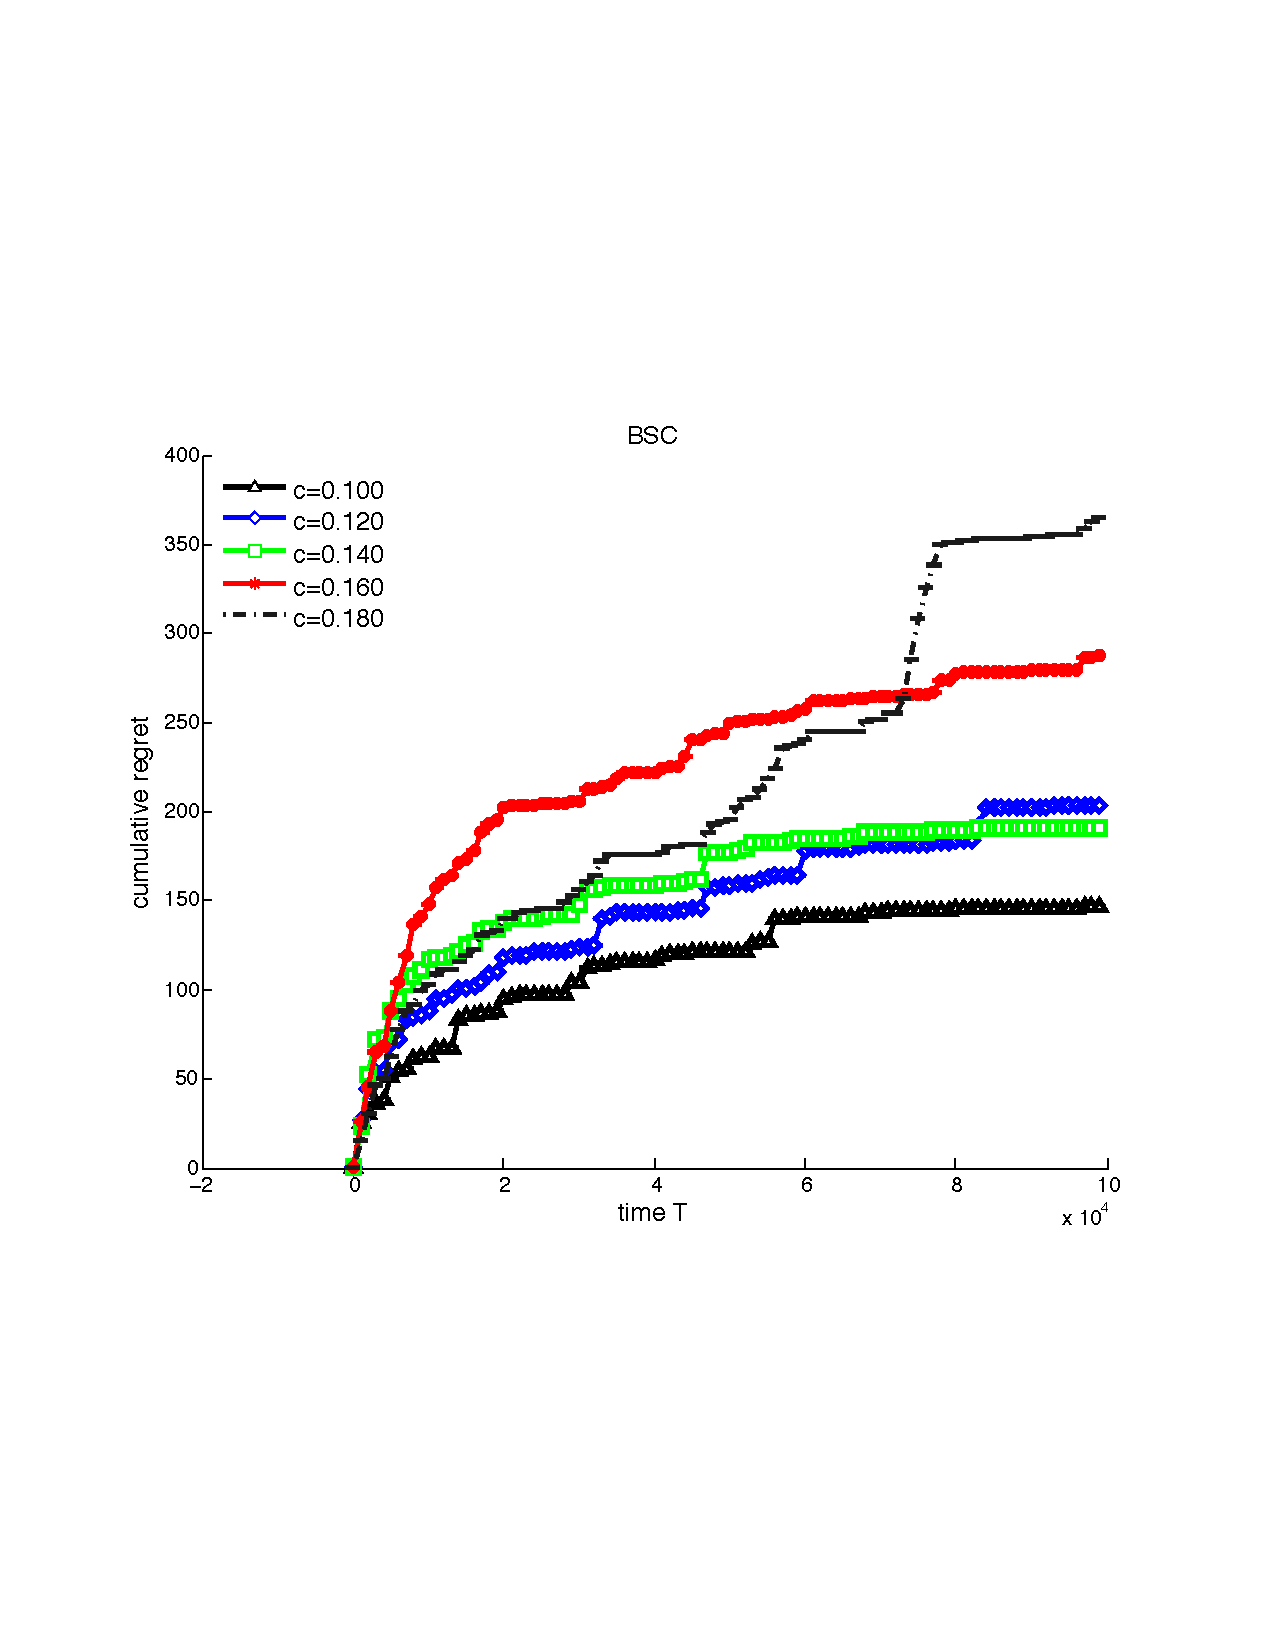
\includegraphics[scale=0.4]{../Simulations/Figures/BSC_SD}
				\vspace{-.3cm}
		\caption{\footnotesize Regret under SD property}
\label{fig:BSC_SD}
	\end{minipage}
	\begin{minipage}{8cm}
		\centering
		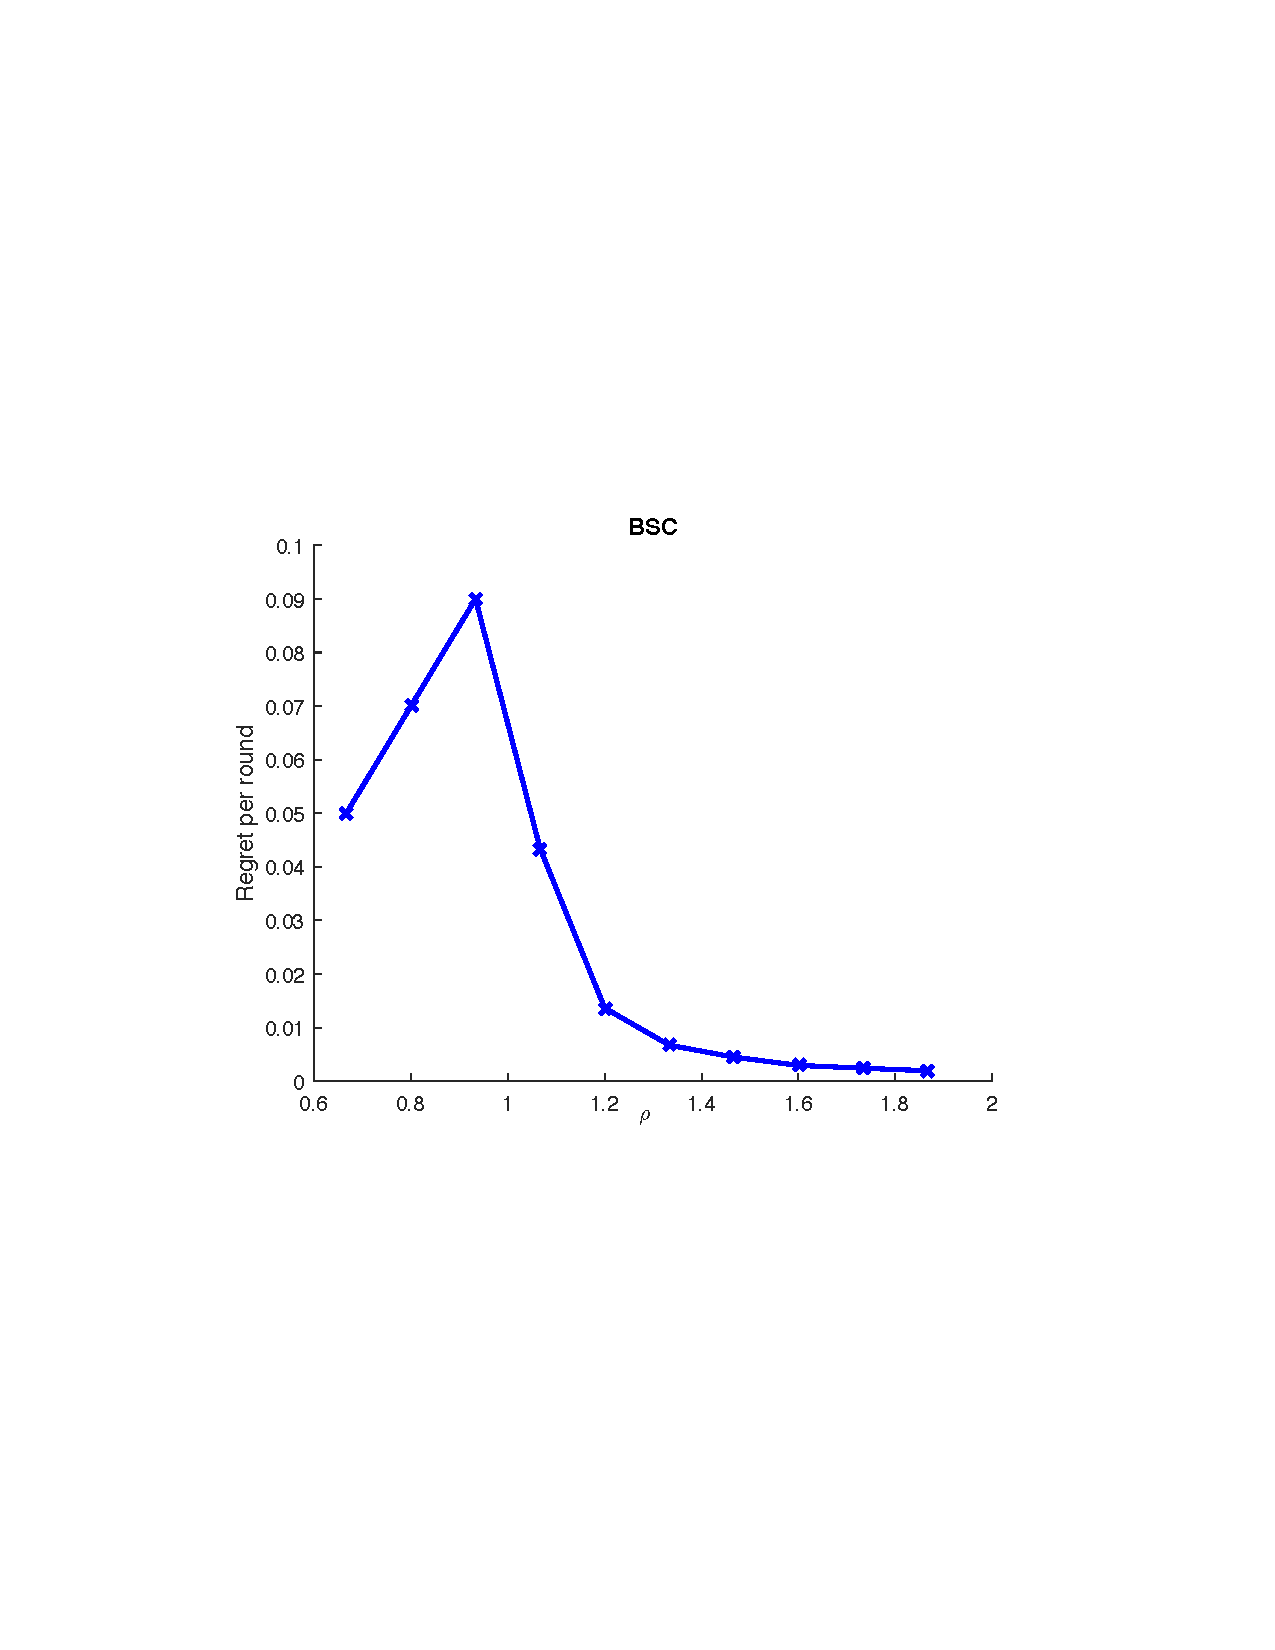
\includegraphics[scale=0.4]{../Simulations/Figures/BSC_WD1}
				\vspace{-.3cm}
		\caption{\footnotesize Regret under varying levels WD condition}
\label{fig:BSC_WD}
	\end{minipage}
%	\begin{minipage}{4cm}
%		\centering
%		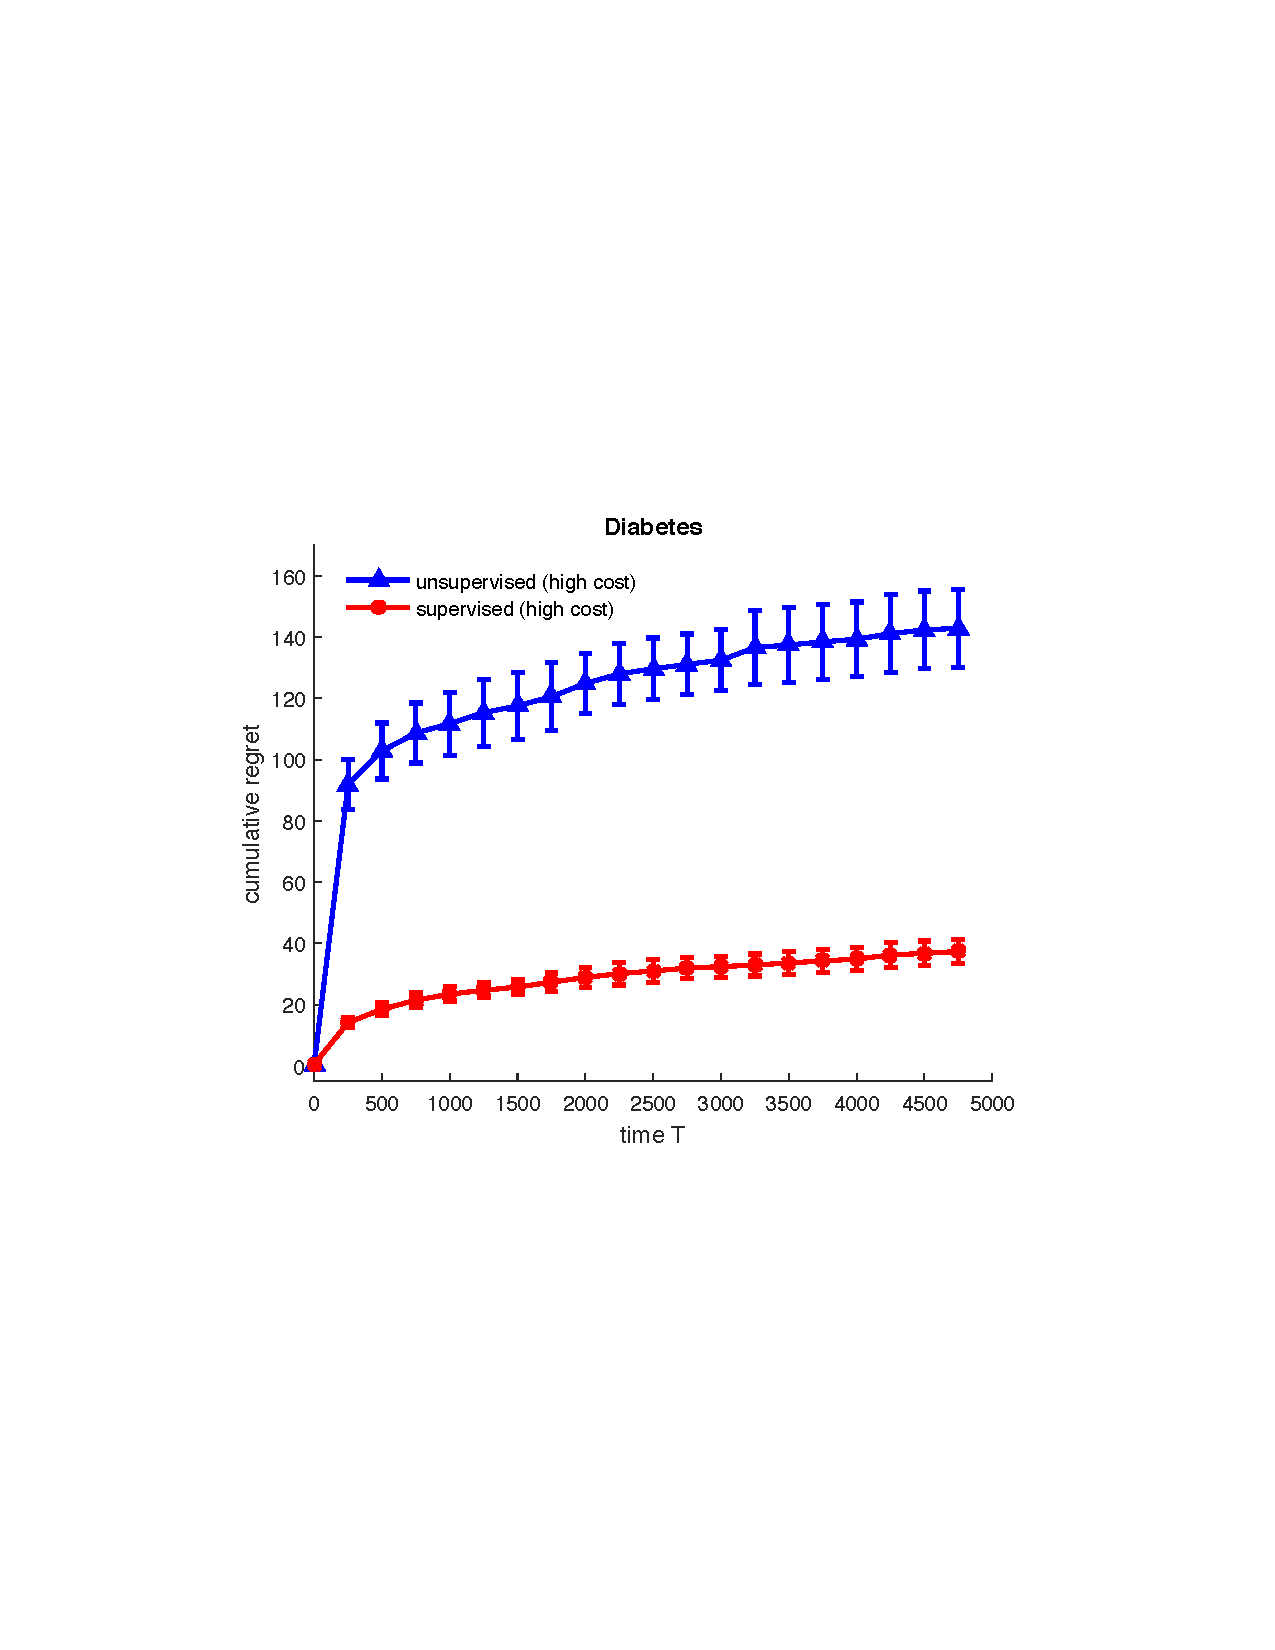
\includegraphics[scale=0.3]{../Simulations/Figures/Diabetes_WD1}
%		\vspace{-.3cm}
%		\caption{\footnotesize {\bf PIMA Diabetes}}
%		\label{fig:Diabetes}
%	\end{minipage}
%	\begin{minipage}{4cm}
%		\centering
%	%	\vspace{.2cm}
%		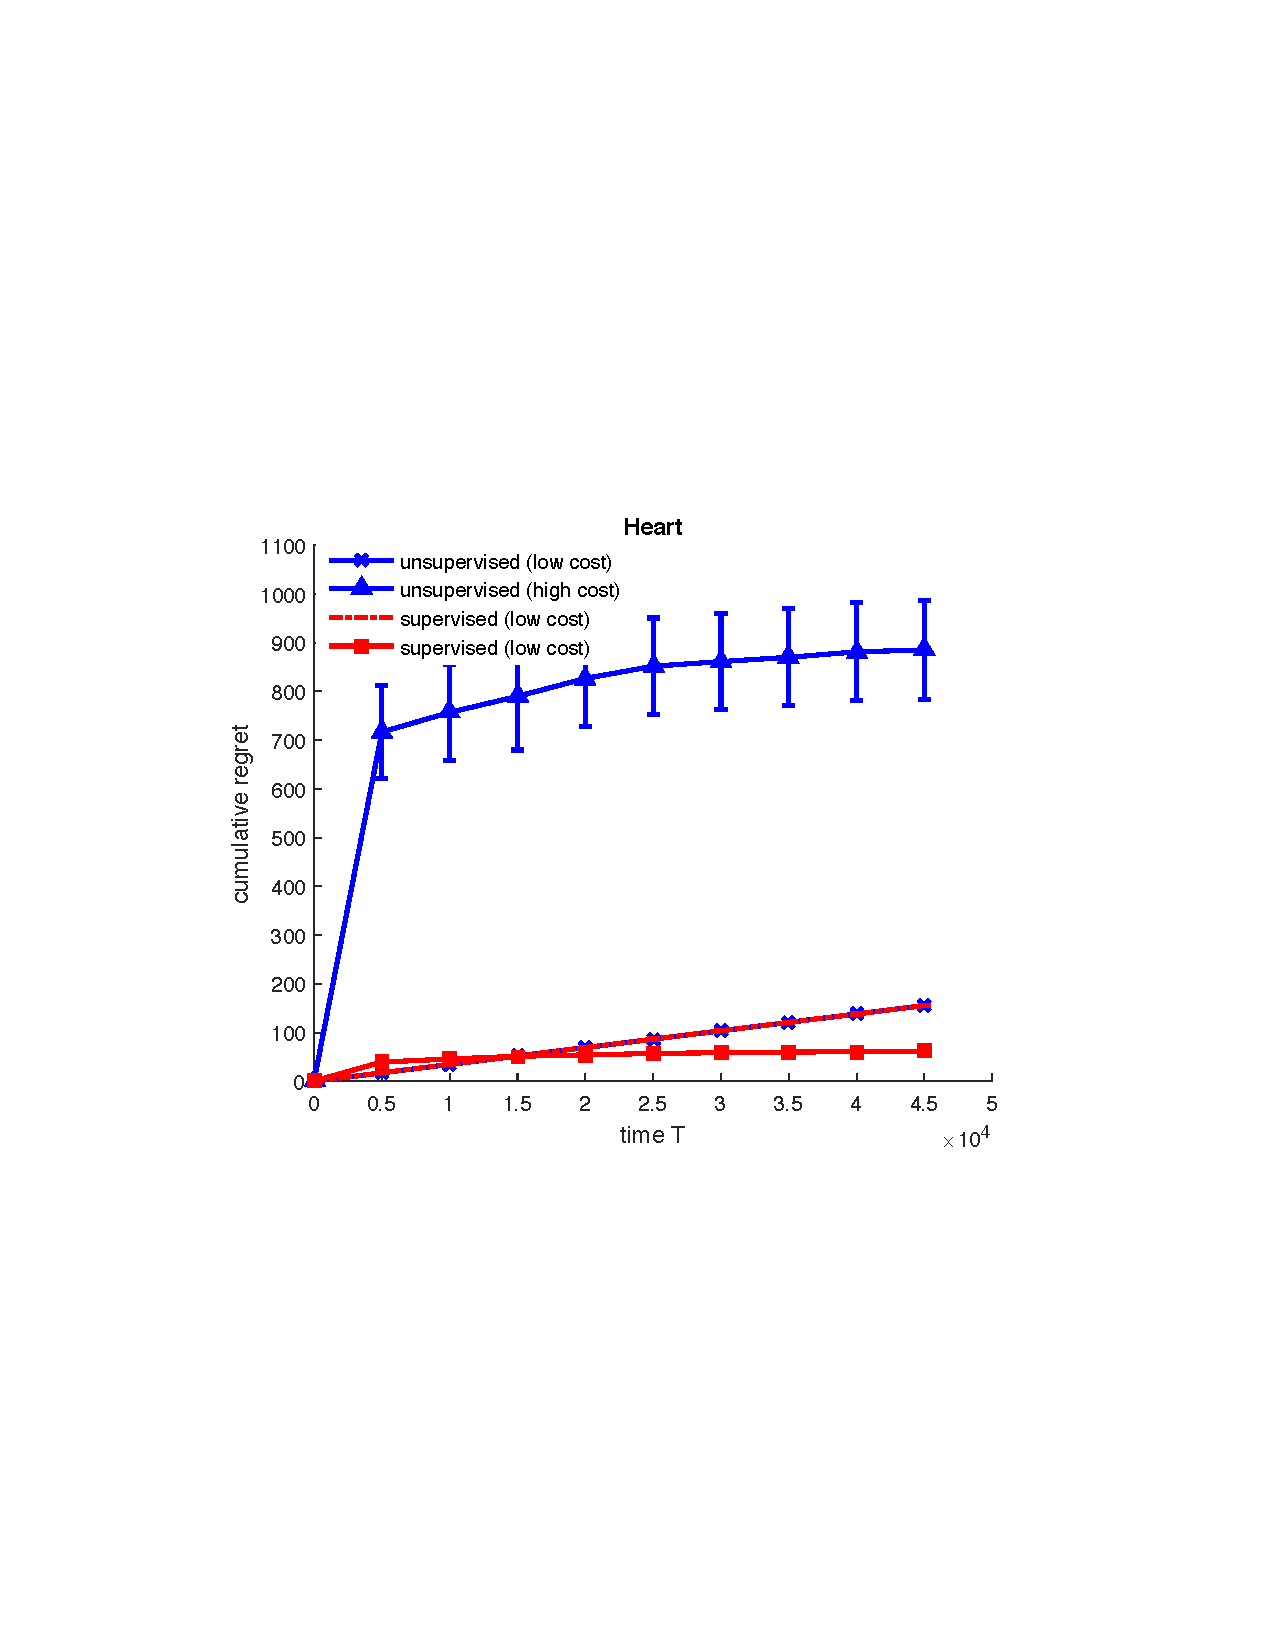
\includegraphics[scale=0.3]{../Simulations/Figures/Heart_WD1}
%%		\vspace{-.5cm}
%		\caption{\footnotesize {\bf Heart Disease}}
%	\label{fig:Heart}
%%\vspace{-.3cm}
%	\end{minipage}
	%\vspace{.3cm}
%
\vspace{5pt}

\noindent
{\footnotesize Fig. \ref{fig:BSC_SD} depicts regret of USS (Alg.~1) on synthetic data. Under SD it is always sublinear regardless of costs/probability. Fig. \ref{fig:BSC_WD} demonstrates phase-transition effect for USS (Alg.~2). Alg.~1 is not plotted here because it fails in this case. As $\rho \rightarrow 1$ (from the right) regret-per-round drastically increases thus validating our theory that WD is a maximal learnable set. 
%, Algorithm \ref{alg:UCB} is applied on BSC data. In Fig. \ref{fig:Diabetes} Algorithm \ref{alg:UCB} and the standard UCB algorithm that uses ground truth are applied on the Diabetes dataset. In Fig. \ref{fig:Heart}, same experiment is repeated on the heart dataset.
}
%\vspace{-15pt}
\end{figure*}
\end{center}

\begin{center}
	\begin{figure*}
		\begin{minipage}{8cm}
			\centering
			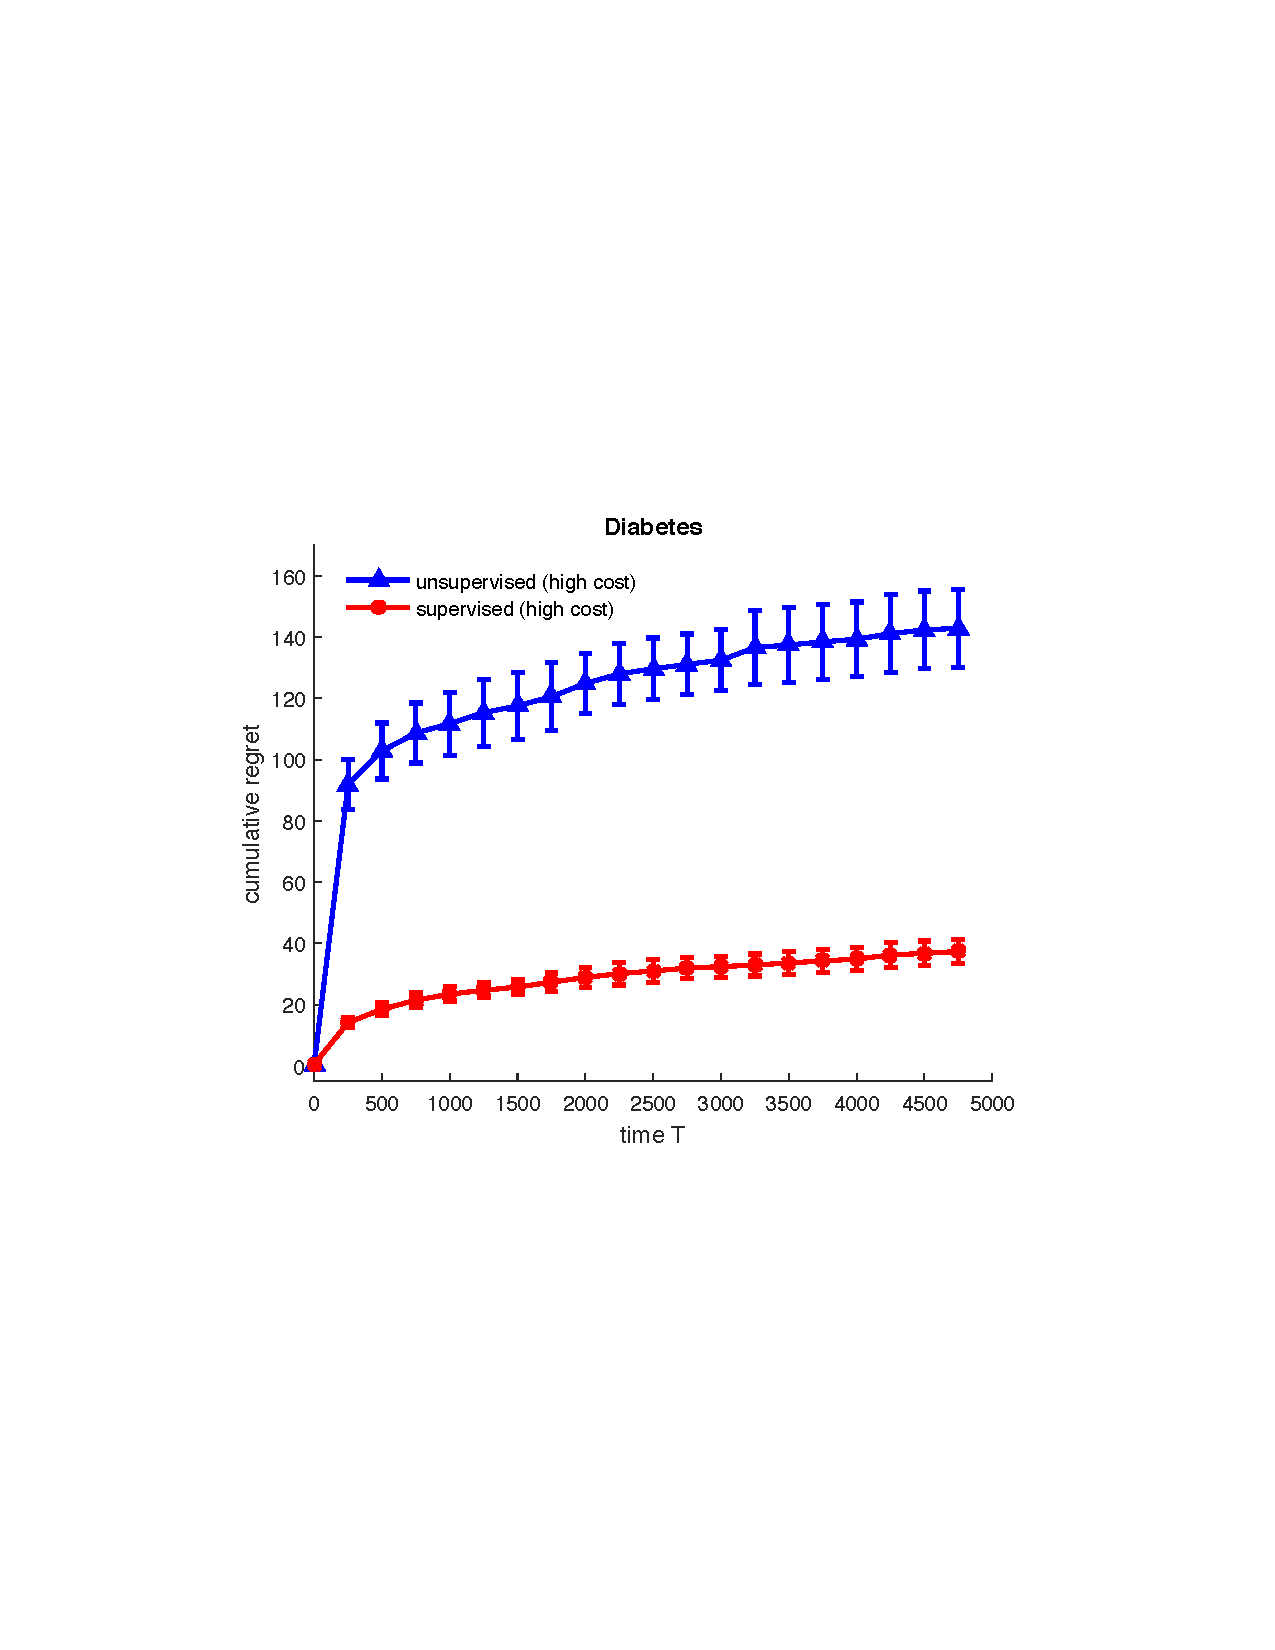
\includegraphics[scale=0.4]{../Simulations/Figures/Diabetes_WD1}
			\vspace{-.3cm}
			\caption{\footnotesize Regret Curves on PIMA Diabetes}
			\label{fig:Diabetes}
		\end{minipage}
		\begin{minipage}{8cm}
			\centering
			%	\vspace{.2cm}
			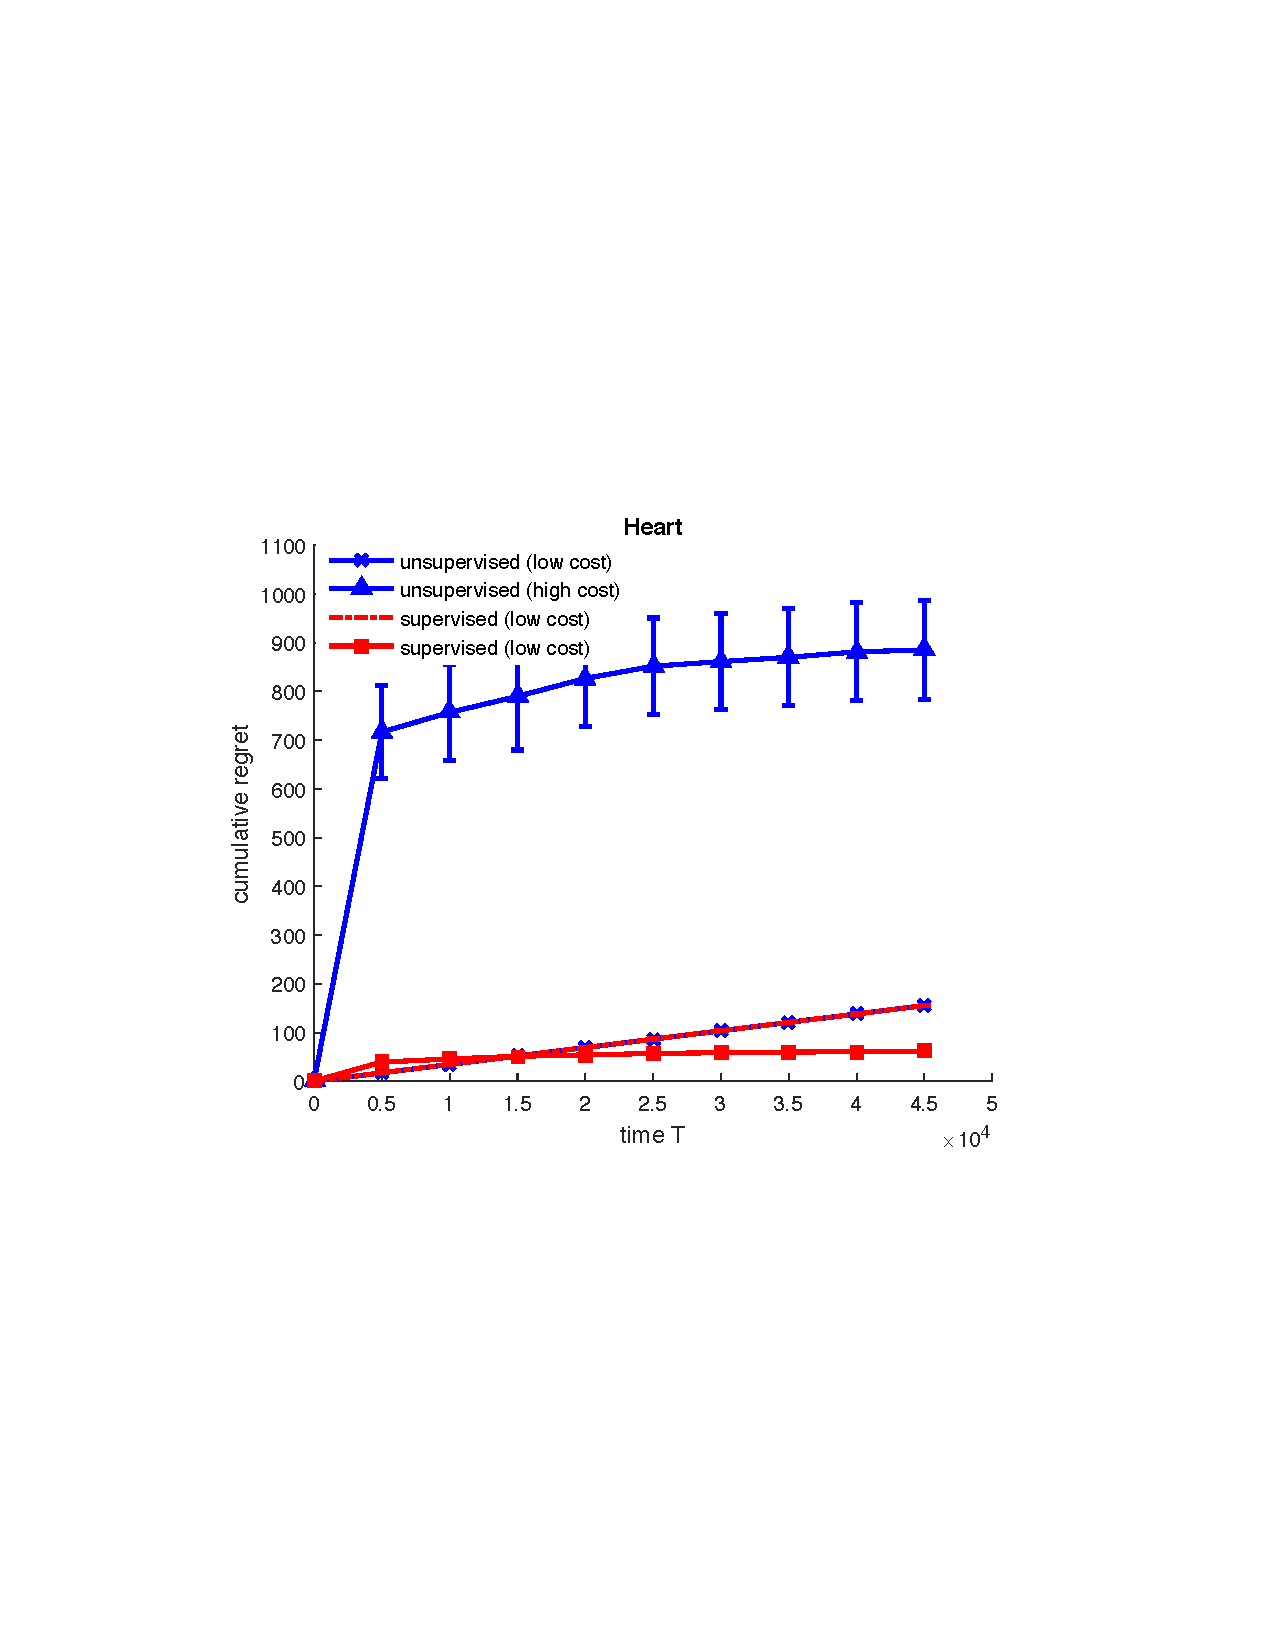
\includegraphics[scale=0.4]{../Simulations/Figures/Heart_WD1}
			\vspace{-.3cm}
			\caption{Regret Curves on Heart Disease}
			\label{fig:Heart}
			%\vspace{-.3cm}
		\end{minipage}
		\vspace{5pt}
		
		\noindent
		{\footnotesize Fig. \ref{fig:Diabetes} and Fig. \ref{fig:Heart} depict performance for real-datasets and presents comparisons against supervised (bandit with ground-truth feedback) scenario. Typically (but not in the worst-case (see Thm~5)), under WD, the unsupervised learning rate is within a constant factor of supervised setting.
			%, Algorithm \ref{alg:UCB} is applied on BSC data. In Fig. \ref{fig:Diabetes} Algorithm \ref{alg:UCB} and the standard UCB algorithm that uses ground truth are applied on the Diabetes dataset. In Fig. \ref{fig:Heart}, same experiment is repeated on the heart dataset.
		}
	\end{figure*}
\end{center}

\noindent
{\bf Testing Learnability:}
We experiment with different USS algorithms on the synthetic dataset. Our purpose is twofold: (a) verify sublinear regret reduction scheme (Alg~1) under SD (b) verify that WD condition is a maximal learnable set. 
Fig.~\ref{fig:BSC_SD} depicts the results of Alg.~\ref{alg:asym} when SD condition is satisfied and shows that we obtain sublinear regret regardless of costs/probabilities. To test WD requirement we parameterize the problem by varying costs. Without loss of generality we fix the cost of sensor 1 to be zero and the total cost of the entire system to be $C_{\mbox{tot}}$. We then vary cost of sensors 2 and 3. %To plot the effect of WD we note from Eq.~\ref{eqn:WD} that for an optimal sensor $i$, $\rho \geq 1$. 
%we must have that if optimal sensor $i <K$ then the ratio,
%$$
%\rho = \min_{i < j} \frac{(c_j - c_i)}{\Pr\{Y^j \neq Y^i\}} \geq 1.
%$$
%This corresponds to the condition that the worst-case marginal-cost to marginal absolute error is bounded by 1.
We test the hypothesis that WD is a maximal learnable set. We enforce Sensor 2 as the optimal sensor and vary the costs so that we continuously pass from the situation where WD holds ($\rho \geq 1$) to the case where WD does not hold ($\rho < 1$). %The optimal arm is correctly identified for all costs. 
Fig.~\ref{fig:BSC_WD} depicts regret-per-round for Alg.~\ref{alg:UCB} and as we can verify there is indeed a transition at $\rho = 1$ . %While for SD condition Alg.~\ref{alg:asym} is superior there is an inherent lack of robustness when SD fails to be satisfied. Consequently,  Alg.~\ref{alg:UCB} is somewhat more robust to relaxation of SD assumption.

\noindent
{\bf Unsupervised vs. Supervised Learning:}
The real datasets provide an opportunity to understand how different types of information can impact performance. We compare USS algorithm (Alg.~2) against a corresponding bandit algorithm where the learner receives feedback. In particular, for each action in each round, in the bandit setting, the learner knows whether or not the corresponding sensor output is correct. We implement the supervised bandit setting by replacing Step 5 in Alg.~2 with estimated marginal error rates. 

We scale costs by means of a tuning parameter (since the costs of features are all greater than one) and consider minimizing a combined objective ($\lambda$ Cost + Error) as stated in Sec.~2. High (low)-values for $\lambda$ correspond to low (high)-budget constraint. If we set a fixed budget of (\$ 50), this corresponds to high-budget (small $\lambda$) and low budget (large $\lambda$) for PIMA Diabetes (3rd test optimal) and Heart Disease (1st test optimal) respectively. Figs~\ref{fig:Diabetes} and \ref{fig:Heart} depicts performance for typical scenarios. We notice that for both high as well as low cost scenarios, while supervised does have lower regret, the USS cummulative regret is also sublinear and within a constant fraction of the supervised case. This is qualititively interesting because these plots demonstrate that (although under WD we do not have uniform learnability), in typical cases, we learn as well as the supervised setting. %as in the supervised bandit setting. In general we emphasize that in many medical and security systems it is often difficult to obtain ground-truth annotatations for examples.



%Our objective is to choose a sensor that minimizes 
%
%We  (Alg.~\ref{alg:UCB}) (unsuprvised) against UCB bandit algorithm that observes reward for each action (supervised). Note that for USS we apply Alg.~\ref{alg:UCB} because the real datasets does not satisfy SD condition and our experience on synthetic data (see Fig.~\ref{fig:BSC_WD}). Our implementation for UCB algorithm is based on modification of Alg.~\ref{alg:UCB}) that keeps track of error rates of each arm by  directly utilizing ground truth $Y$ rather than pairwise-disagreements (Step 5 in Alg.~\ref{alg:UCB}). We benchmark the performance with respect to a budget constrained problem, where the objective is to pick a sensor that minimizes error with respect to a budget constraint. We consider both high and low available budget situations. For Heart and Diabetes datasets a low budget is about (\$ 10). We note from the error probabilities in Table~\ref{tab:error_stats} that the optimal sensor in such a situation is Sensor 1. On the other hand for a budget of about (\$ 50) the optimal sensor for Diabetes dataset is Sensor 3, while for the Heart dataset it is Sensor 2. To map this to our setting we consider an equivalent error-cost tradeoff objective ($\lambda$ Cost + Error) with an appropriate scaling parameter $\lambda$ so that it leads to the same sensor choice based on Eq.~\ref{eqn:interp_opt} as in the constrained one. We then compare supervised and unsupervised scenarios in Figs~\ref{fig:Diabetes} and \ref{fig:Heart} for real datasets. We notice that for both high as well as low cost scenarios, while supervised does have lower regret, the cummulative regret is also sublinear and within a constant fraction of the regret for unsupervised case. This is qualititively interesting because these plots demonstrate that (although under WD we do not have uniform learnability) in typical cases we learn in unsupervised setting as in the supervised bandit setting. In general we emphasize that in many medical and security systems it is often difficult to obtain ground-truth annotatations for examples.


%Fo the synthetic experiments we set $c_1=0$ and $c_2+c_3=0.4$ while varying $c_2$ from $0.1$ to $0.29$. The optimal action in this setup is $2$. In Figure \ref{fig:BSC_SD} we applied Algorithm \ref{alg:asym} on BSC data that satisfies SD property. As seen, the algorithm learns the optimal arm for all values of $c_2$. In Fig. ~\ref{fig:BSC_WD} 
%we applied Alg. ~\ref{alg:UCB} on BSC data, where $x$-axis in the figure is the ratio
%\[R= \frac{0.4 - c_2}{\Pr\{Y^2 \neq Y^3\}}\]
%and $y$-axis is the regret per round. As shown, regret per round is small when $R>1$, whereas it is high for $R<1$. This observation follows by applying definition of (\ref{dfn:WDP})- when $R>1$, the setup satisfies the WD property and the algorithm identifies the optimal action, whereas when $R<1$ the setup violates the WD property and the algorithm cannot identify the optimal arm resulting in high regret per round. This validates the learnability under the WD property. 

%In figure \ref{fig:Diabetes}, we apply Algorithm $2$ and the standard UCB algorithm on the Diabetes dataset. In applying the standard using algorithm, we use the true label in each round to get the loss for the action played. The regret plots corresponding to the Algorithm $2$ are labeled as unsupervised and that corresponding to standard UCB as supervised in the figure. We consider two values for trade-off factor, $\lambda=0.001$ and $\lambda=0.015$. In the first case, accuracy is given higher weight and action $3$ is optimal, in the second cost factor becomes dominant and action $1$ is optimal. When action $3$ is optimal, the performance of both the supervised and unsupervised methods are almost identical. When action $1$ is optimal. As expected, the performance of unsupervised method is better than the supervised method, but unsupervised method learns the optimal arms almost after the same number of rounds as the supervised method though it incurs high regret in the initial rounds.


%In figure \ref{fig:Heart} we again apply Algorithm $2$ on the standard UCB algorithm on the heart dataset. We set $\lambda=0.05$ for which action $1$ is optimal. The two corresponding plots are labeled as unsupervised and supervised in the figure. We also plot the regret obtained when noisy labels are input to the 
%the standard UCB algorithm instead of the true labels. This plot is labeled as supervised (noisy) in the figure which is obtained when each label is flipped by probability $0.2$. As seen, the regret performance of the supervised method deteriorates as label gets noisier. 


%and the average is shown in figures (\ref{fig:BSC1}-\ref{fig:Heart}) with $95\%$ confidence bounds. The left Figure in\ref{fig: BSC1} we applied Algorithm \ref{alg:asym} on BSC data that satisfies SD property. As see, the algorithm learns the optimal arm. In Figure \ref{fig:BSC2} 
%we applied Algorithm \ref{alg:UCB} on BSC data where we fixed $c_1=0$ and $c_2+c_3=0.3$ while varying $c_2$ between $0.1$ $0.18$. For all the cost values, arm $2$ is optimal. When $c_2 \in \{0.1, 0.12,  0.14\}$ the weak dominance property is satisfied and the algorithm learns the optimal arm. For values $c_2 \in \{0.16, 0.18\}$ weak dominance property is violated we get linear regret as shown in the plots. In figure  \ref{fig:BSC3} we use the standard UCB algorithm that has access to the true labels and knows the if a sensor made error. As seen this setting learns much faster than than compared to unsupervised algorithm shown in figure \ref{fig:BSC1} and \ref{fig:BSC2}. In figure we apply Algorithm \ref{algo:UCB} on diabetes dataset varying the trade-off factor $\lambda$. In the regions where WD property holds, the algorithm identifies the optimal arm.